%!TEX root = ../Compte-rendu.tex
\section{Caractéristiques communes aux trois expériences}
\subsection{Environnement}
Une grille de taille $50 \times 50$ avec 3 obstacles de taille $5 \times 5$
disposés aléatoirement sur la grille. Un agent (une tortue) positionné aléatoirement
sur cette même grille. Selon les expériences un ou plusieurs débris sont disposés 
aléatoirement sur la grille.
\subsection{Mesure utilisée}
Pour pouvoir comparer les résultats entre les stratégies nous avons défini
la mesure suivante : $$\cfrac{\text{Nombre de \emph{ticks}}}{\text{Nombre de débris collectés}}$$
Cette mesure permet de savoir combien, en moyenne, de \emph{ticks} sont nécessaires
pour la collecte d'un débris.
\section{Un seul débris}
%!TEX root = ../../Compte-rendu.tex
%\subsection{Description}
La seconde comparaison sera faite avec cent débris répartis uniformément.
%!TEX root = ../../Compte-rendu.tex


\begin{figure}[H]
	\begin{center}
		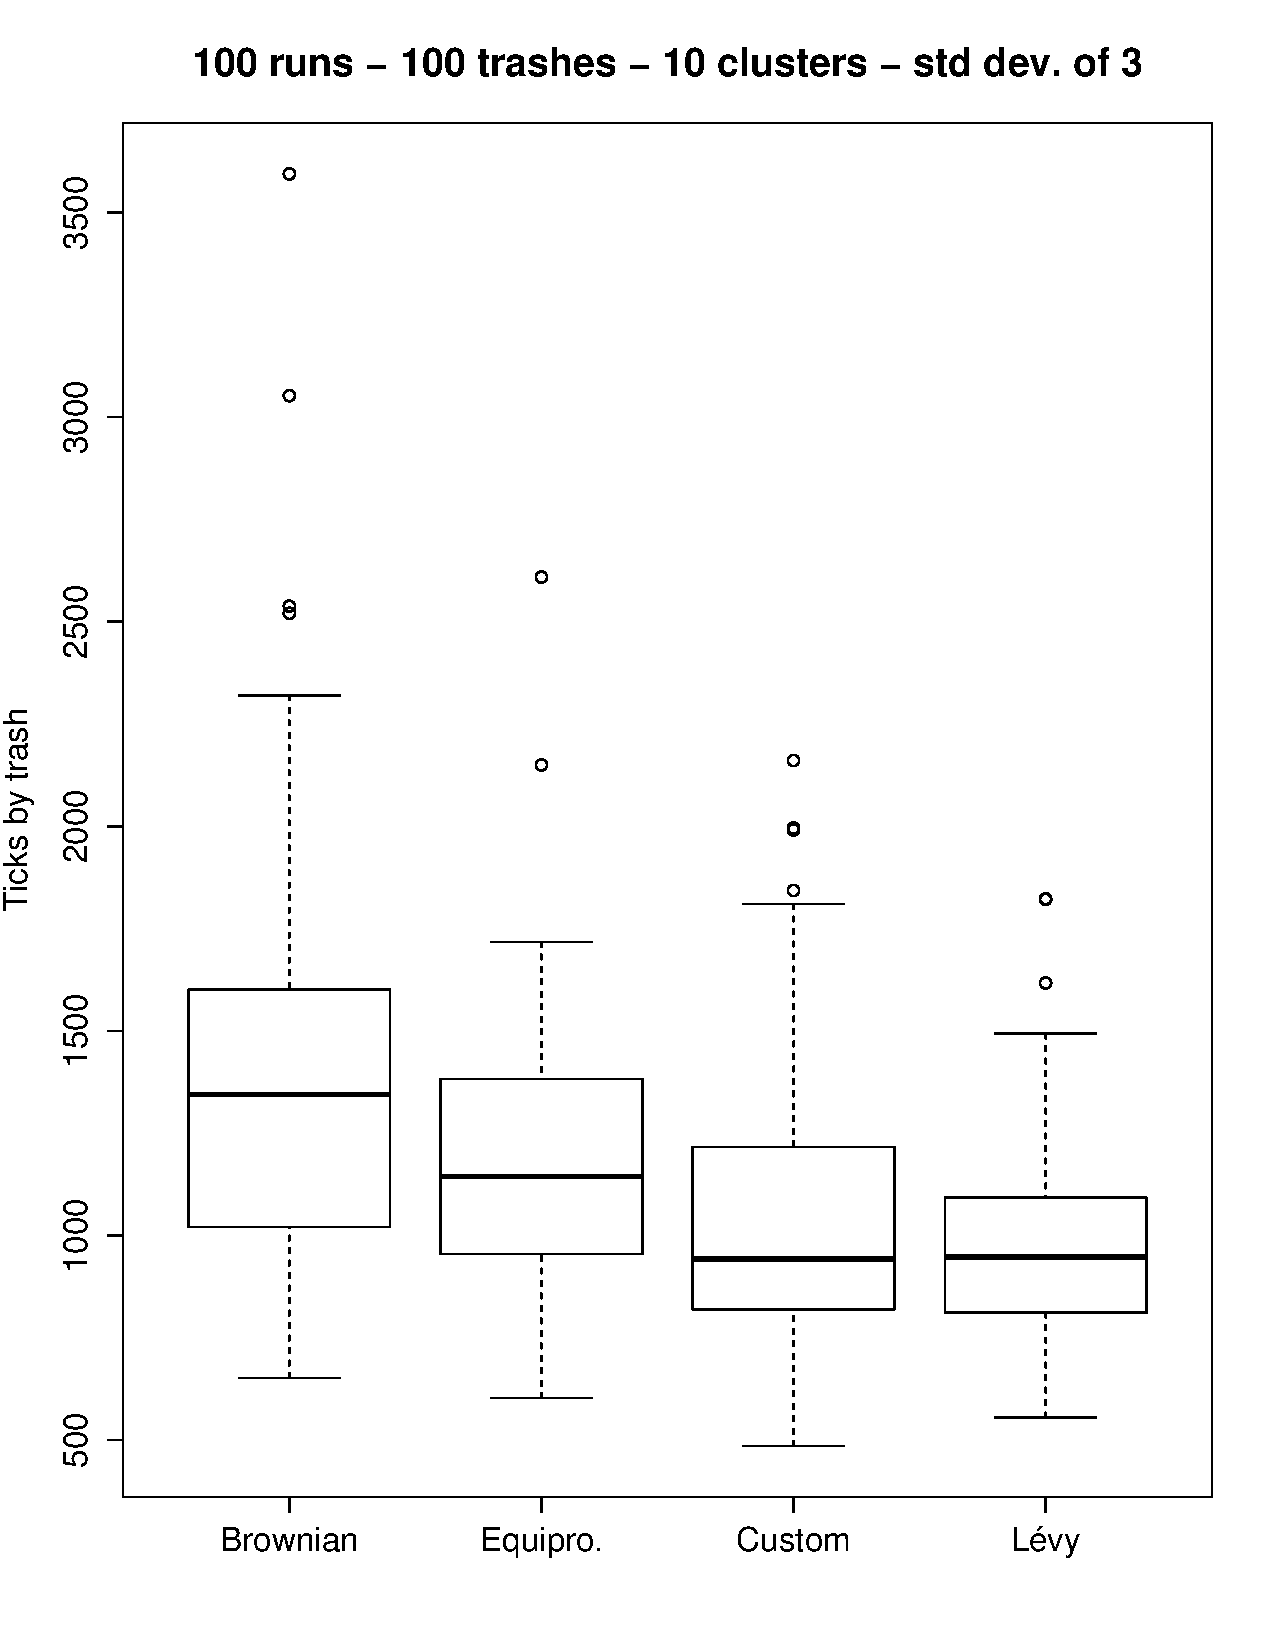
\includegraphics[height=10cm]{diagrams/100Tr10Clts_all.pdf}
		\caption{Résultat des mesures pour 100 débris distribué en 10 clusters (écart-type 3)}
		\label{fig:100Trashes_10Clusters}
	\end{center}
\end{figure}

Nous avons pour les différentes stratégies les statistiques suivantes :

\begin{figure}[H]
	\begin{center}
		\begin{tabular}{| c || c | c | c | c | }
			\hline
			&Brown.&Equi.&Custom&Lévy \\
			\hline
			\hline
			md&1344&1144&942&947\\
			mean&1388&1187&1053&984\\
			min & 652 & 602 & 485 & 555 \\
			max & 3595 & 2609 & 2161 & 1823 \\
			sd&491&318&344&256\\
			p-val&$\ll 5\%$&$\ll 5\%$&$\ll 5\%$&$\ll 5\%$\\
			\hline
		\end{tabular}
		\caption{Statistiques pour 100 débris distribué en 10 clusters (écart-type 3)}
	\end{center}
\end{figure}


Nous pouvons constater que la stratégie Custom a une médiane très
légèrement meilleure à la stratégie Lévy, néanmoins cette première
est moins fiable, c'est à dire que celle-ci a plus de chance de produire
des résultats bien moins bons que le Lévy.

Nous pouvons aussi voir que la stratégie Custom perd en fiabilité
alors que la stratégie Equiprobable, elle, en gagne.

\section{Cent débris uniformément répartis}
%!TEX root = ../../Compte-rendu.tex
%\subsection{Description}
La seconde comparaison sera faite avec cent débris répartis uniformément.
%!TEX root = ../../Compte-rendu.tex


\begin{figure}[H]
	\begin{center}
		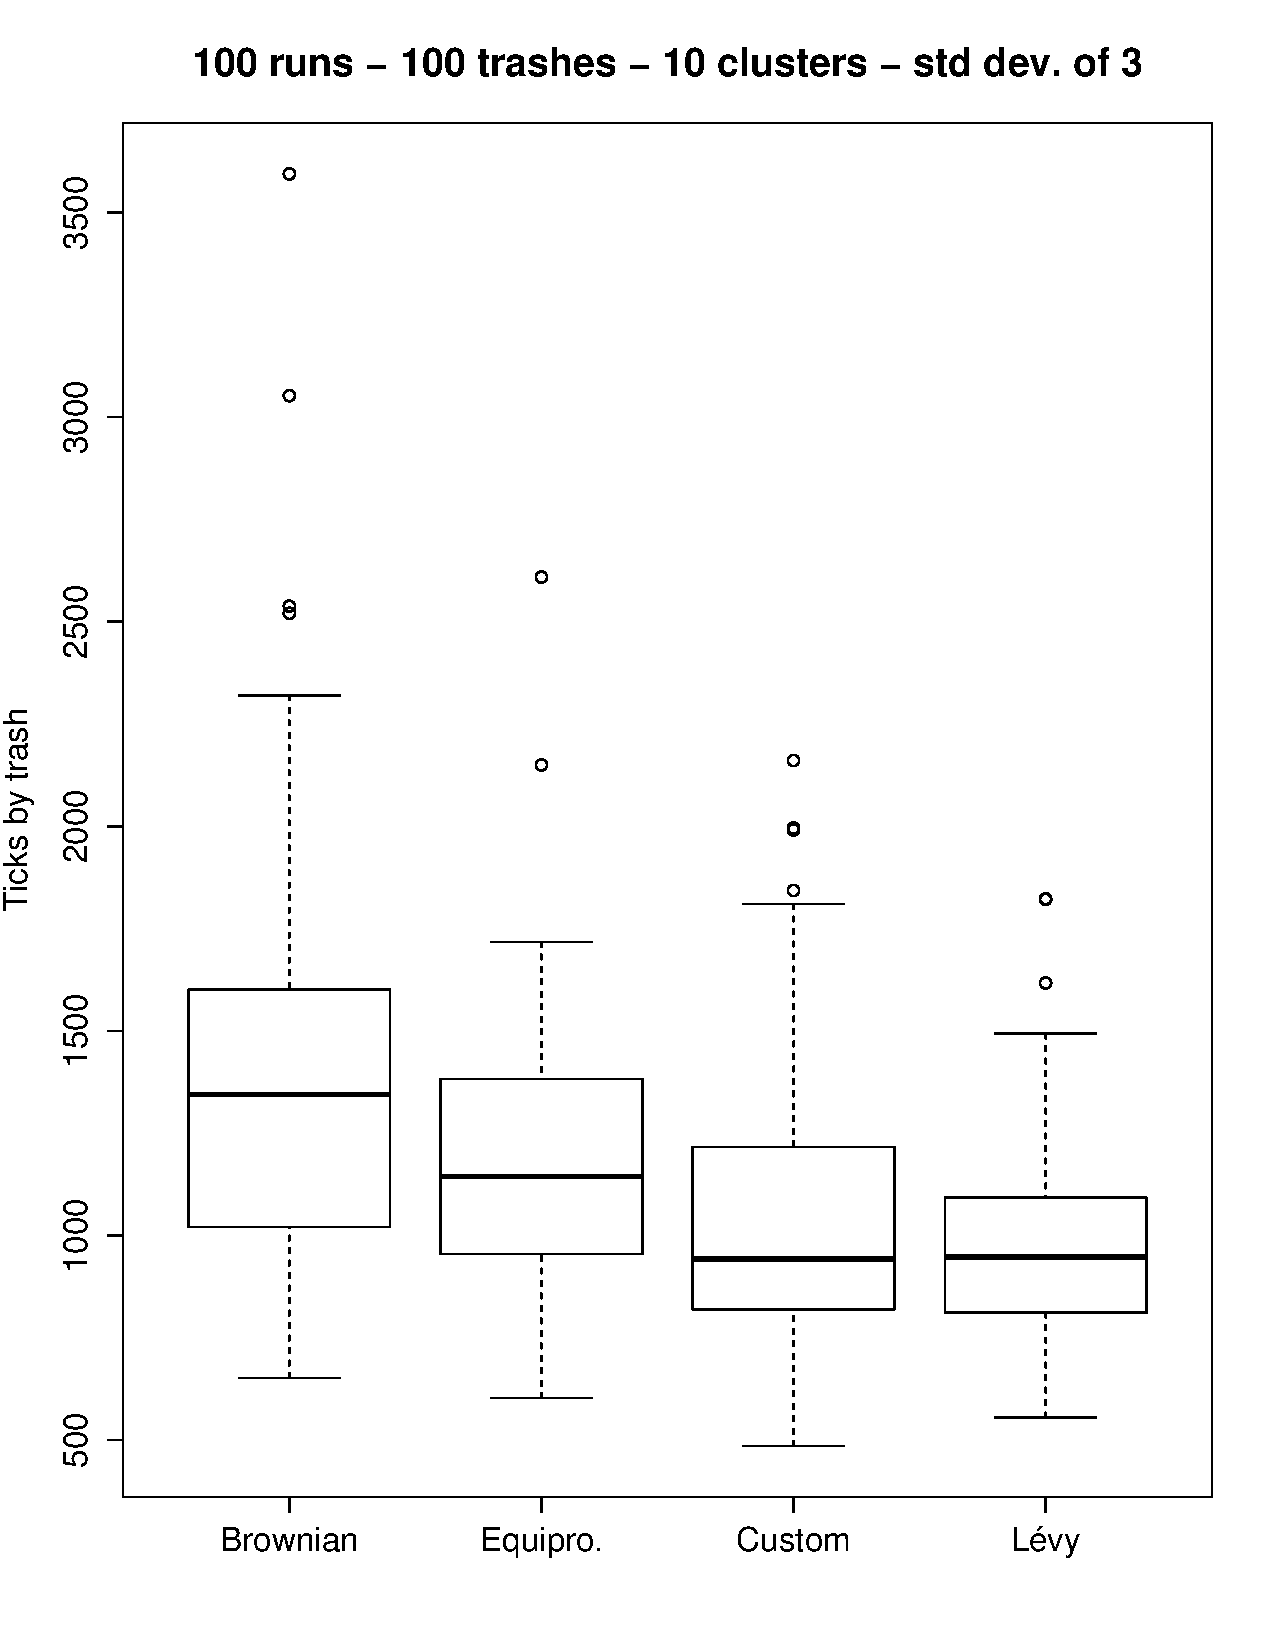
\includegraphics[height=10cm]{diagrams/100Tr10Clts_all.pdf}
		\caption{Résultat des mesures pour 100 débris distribué en 10 clusters (écart-type 3)}
		\label{fig:100Trashes_10Clusters}
	\end{center}
\end{figure}

Nous avons pour les différentes stratégies les statistiques suivantes :

\begin{figure}[H]
	\begin{center}
		\begin{tabular}{| c || c | c | c | c | }
			\hline
			&Brown.&Equi.&Custom&Lévy \\
			\hline
			\hline
			md&1344&1144&942&947\\
			mean&1388&1187&1053&984\\
			min & 652 & 602 & 485 & 555 \\
			max & 3595 & 2609 & 2161 & 1823 \\
			sd&491&318&344&256\\
			p-val&$\ll 5\%$&$\ll 5\%$&$\ll 5\%$&$\ll 5\%$\\
			\hline
		\end{tabular}
		\caption{Statistiques pour 100 débris distribué en 10 clusters (écart-type 3)}
	\end{center}
\end{figure}


Nous pouvons constater que la stratégie Custom a une médiane très
légèrement meilleure à la stratégie Lévy, néanmoins cette première
est moins fiable, c'est à dire que celle-ci a plus de chance de produire
des résultats bien moins bons que le Lévy.

Nous pouvons aussi voir que la stratégie Custom perd en fiabilité
alors que la stratégie Equiprobable, elle, en gagne.

\section{Cent débris répartis en dix clusters}
%!TEX root = ../../Compte-rendu.tex
%\subsection{Description}
La seconde comparaison sera faite avec cent débris répartis uniformément.
%!TEX root = ../../Compte-rendu.tex


\begin{figure}[H]
	\begin{center}
		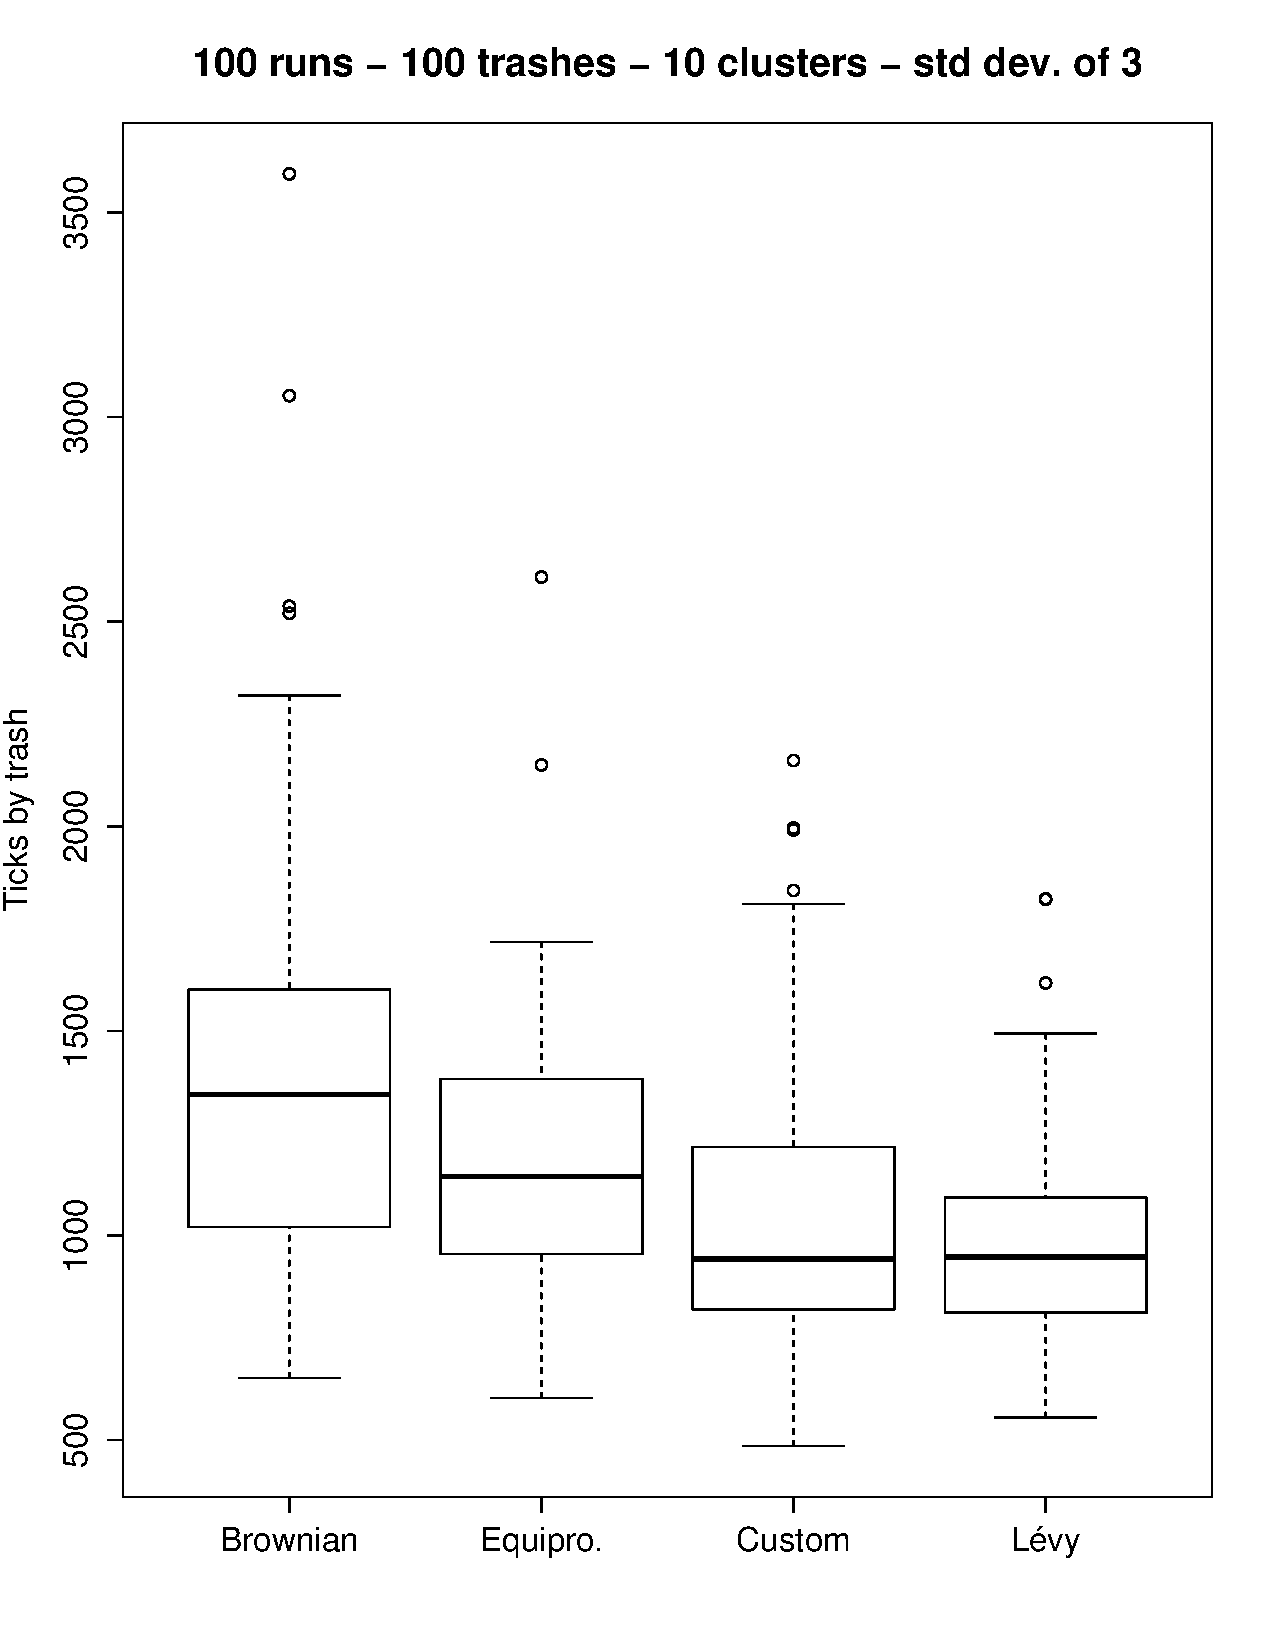
\includegraphics[height=10cm]{diagrams/100Tr10Clts_all.pdf}
		\caption{Résultat des mesures pour 100 débris distribué en 10 clusters (écart-type 3)}
		\label{fig:100Trashes_10Clusters}
	\end{center}
\end{figure}

Nous avons pour les différentes stratégies les statistiques suivantes :

\begin{figure}[H]
	\begin{center}
		\begin{tabular}{| c || c | c | c | c | }
			\hline
			&Brown.&Equi.&Custom&Lévy \\
			\hline
			\hline
			md&1344&1144&942&947\\
			mean&1388&1187&1053&984\\
			min & 652 & 602 & 485 & 555 \\
			max & 3595 & 2609 & 2161 & 1823 \\
			sd&491&318&344&256\\
			p-val&$\ll 5\%$&$\ll 5\%$&$\ll 5\%$&$\ll 5\%$\\
			\hline
		\end{tabular}
		\caption{Statistiques pour 100 débris distribué en 10 clusters (écart-type 3)}
	\end{center}
\end{figure}


Nous pouvons constater que la stratégie Custom a une médiane très
légèrement meilleure à la stratégie Lévy, néanmoins cette première
est moins fiable, c'est à dire que celle-ci a plus de chance de produire
des résultats bien moins bons que le Lévy.

Nous pouvons aussi voir que la stratégie Custom perd en fiabilité
alors que la stratégie Equiprobable, elle, en gagne.